\chapter{Proposed Solutions}
\label{method}

\section{Sci-Genie : Search Engine Harnessing Structure Of Scientific Research}
\begin{figure}[h]
    \centering
    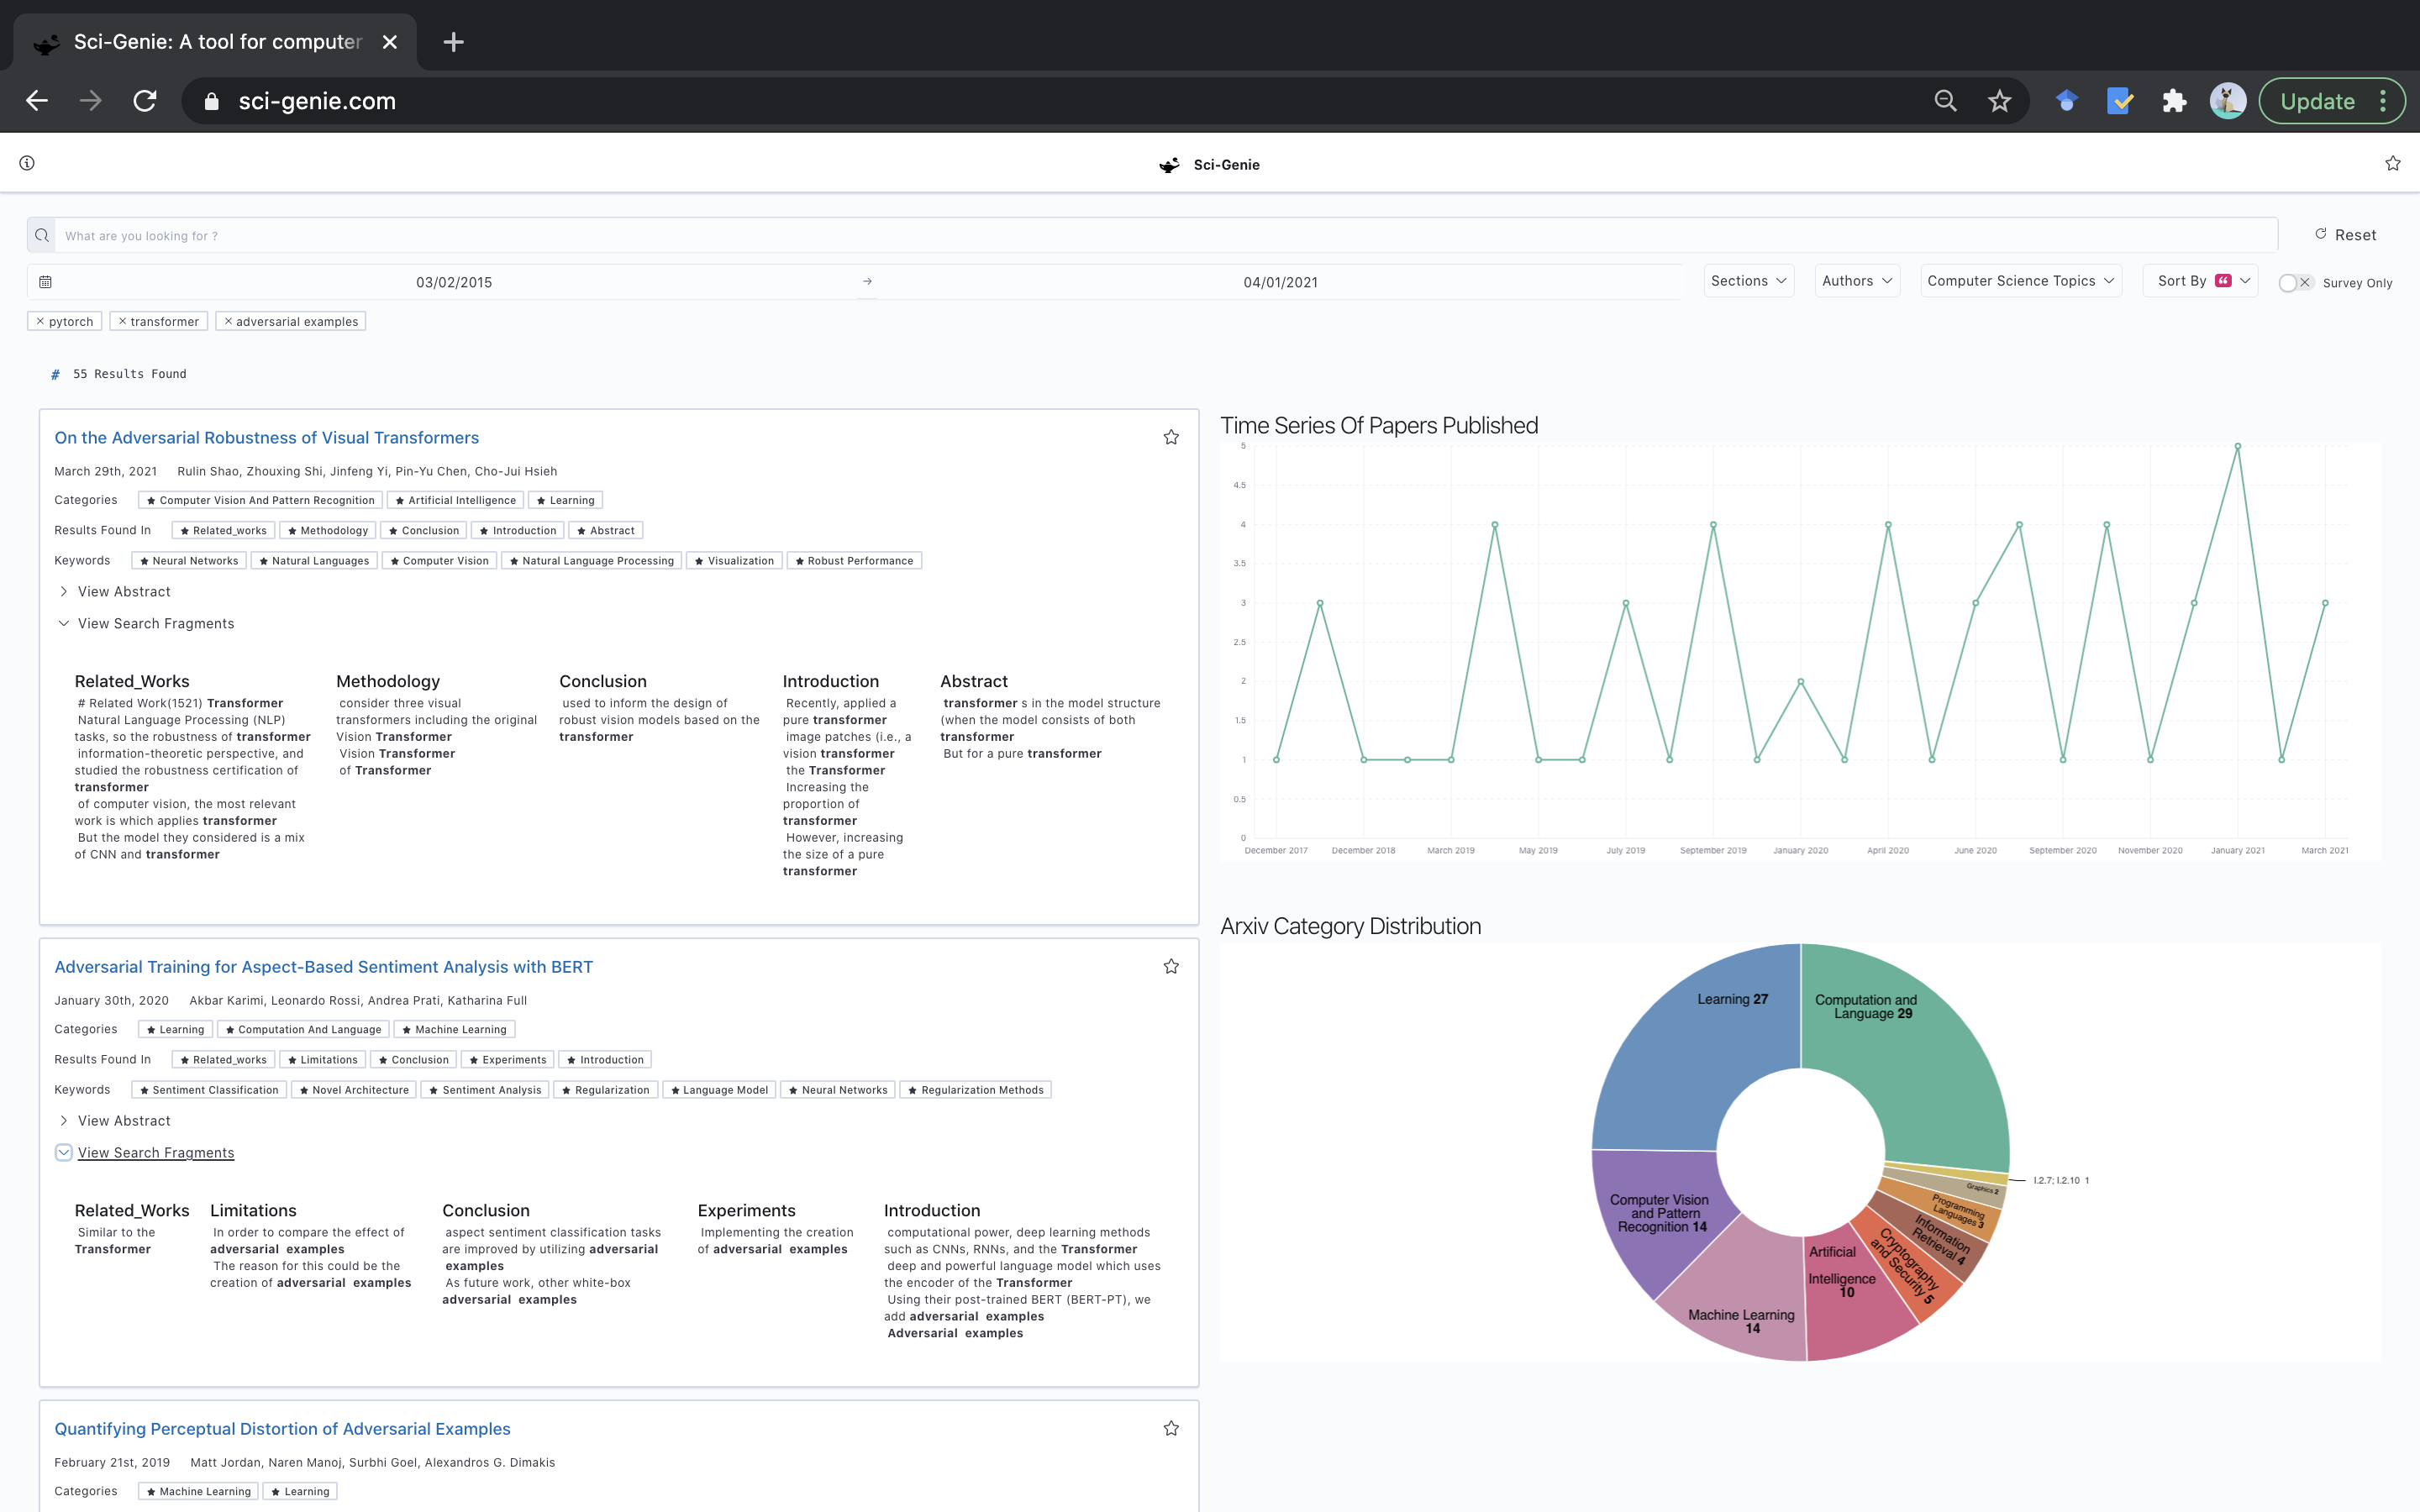
\includegraphics[width=\maxwidth{\textwidth}]{src/images/sci-genie-context-exp.png}
    \caption{Search Results With Context For Query \textit{pytorch, transformer, adversarial examples} Using Sci-Genie}
    \label{figure\arabic{figurecounter}}
\end{figure}
\refstepcounter{figurecounter}

Sci-Genie is a prototype search engine over CS ArXiv. 
Sci-Genie indexes the hierarchical structure of Computer Science research papers 
to provide more context to search results fragments. 
Sci-Genie's content mining engine also classifies a paper's ontology using a SOTA ontology classification model
developed by \cite{salatino2020ontology}. The mined ontology helps create a "Controlled Vocabulary" for filtering search results. 

\section{Sci-Genie-Extension: In-Browser Extension To Augment Information About Research }

\begin{figure}[h]
    \centering
    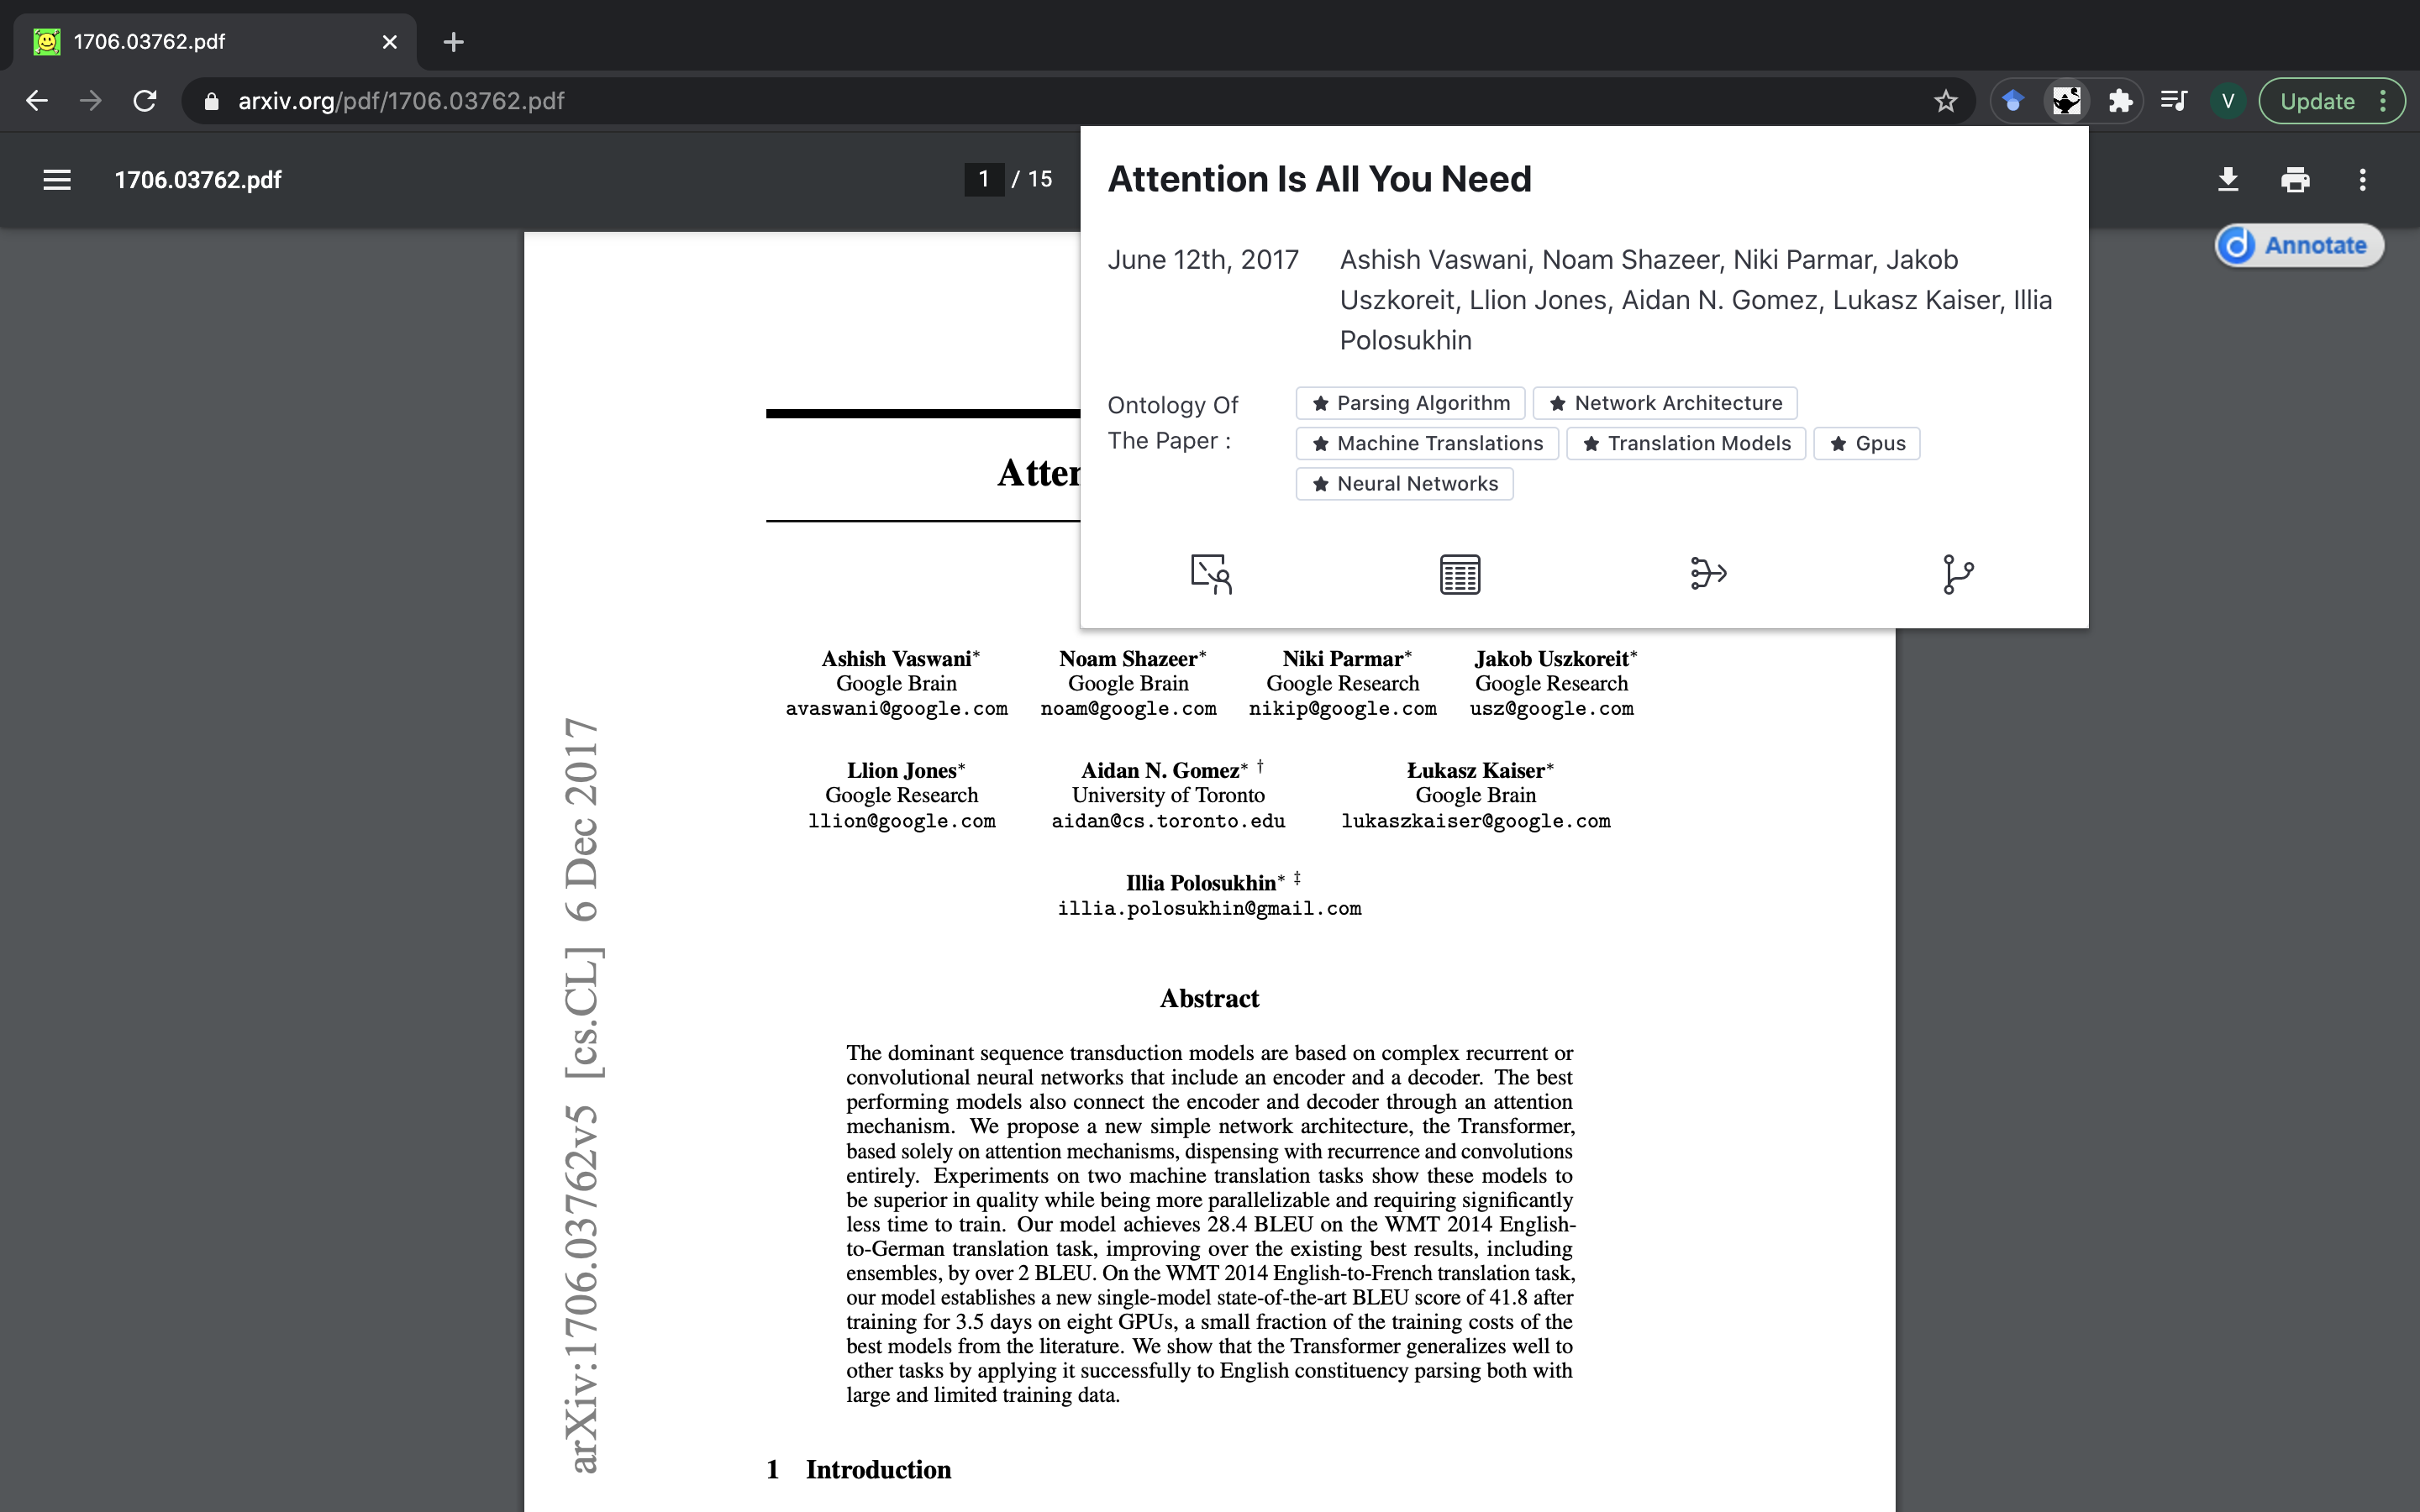
\includegraphics[width=\maxwidth{\textwidth}]{src/images/sci-genie-ext-exp.png}
    \caption{ Sci-Genie Browser Plugin}
    \label{figure\arabic{figurecounter}}
\end{figure}
\refstepcounter{figurecounter}

Sci-Genie, at its core, holds research from CS ArXiv, Tables from the paper mined from CS ArXiv and 
6.5M papers filtered from the Semantic Scholar Open Research Corpus\parencite{ammar-etal-2018-construction}.
The Semantic Scholar Open Research Corpus helps create a citation graph supporting information augmentation for the browser plugin. 

\begin{figure}[h]
    \centering
    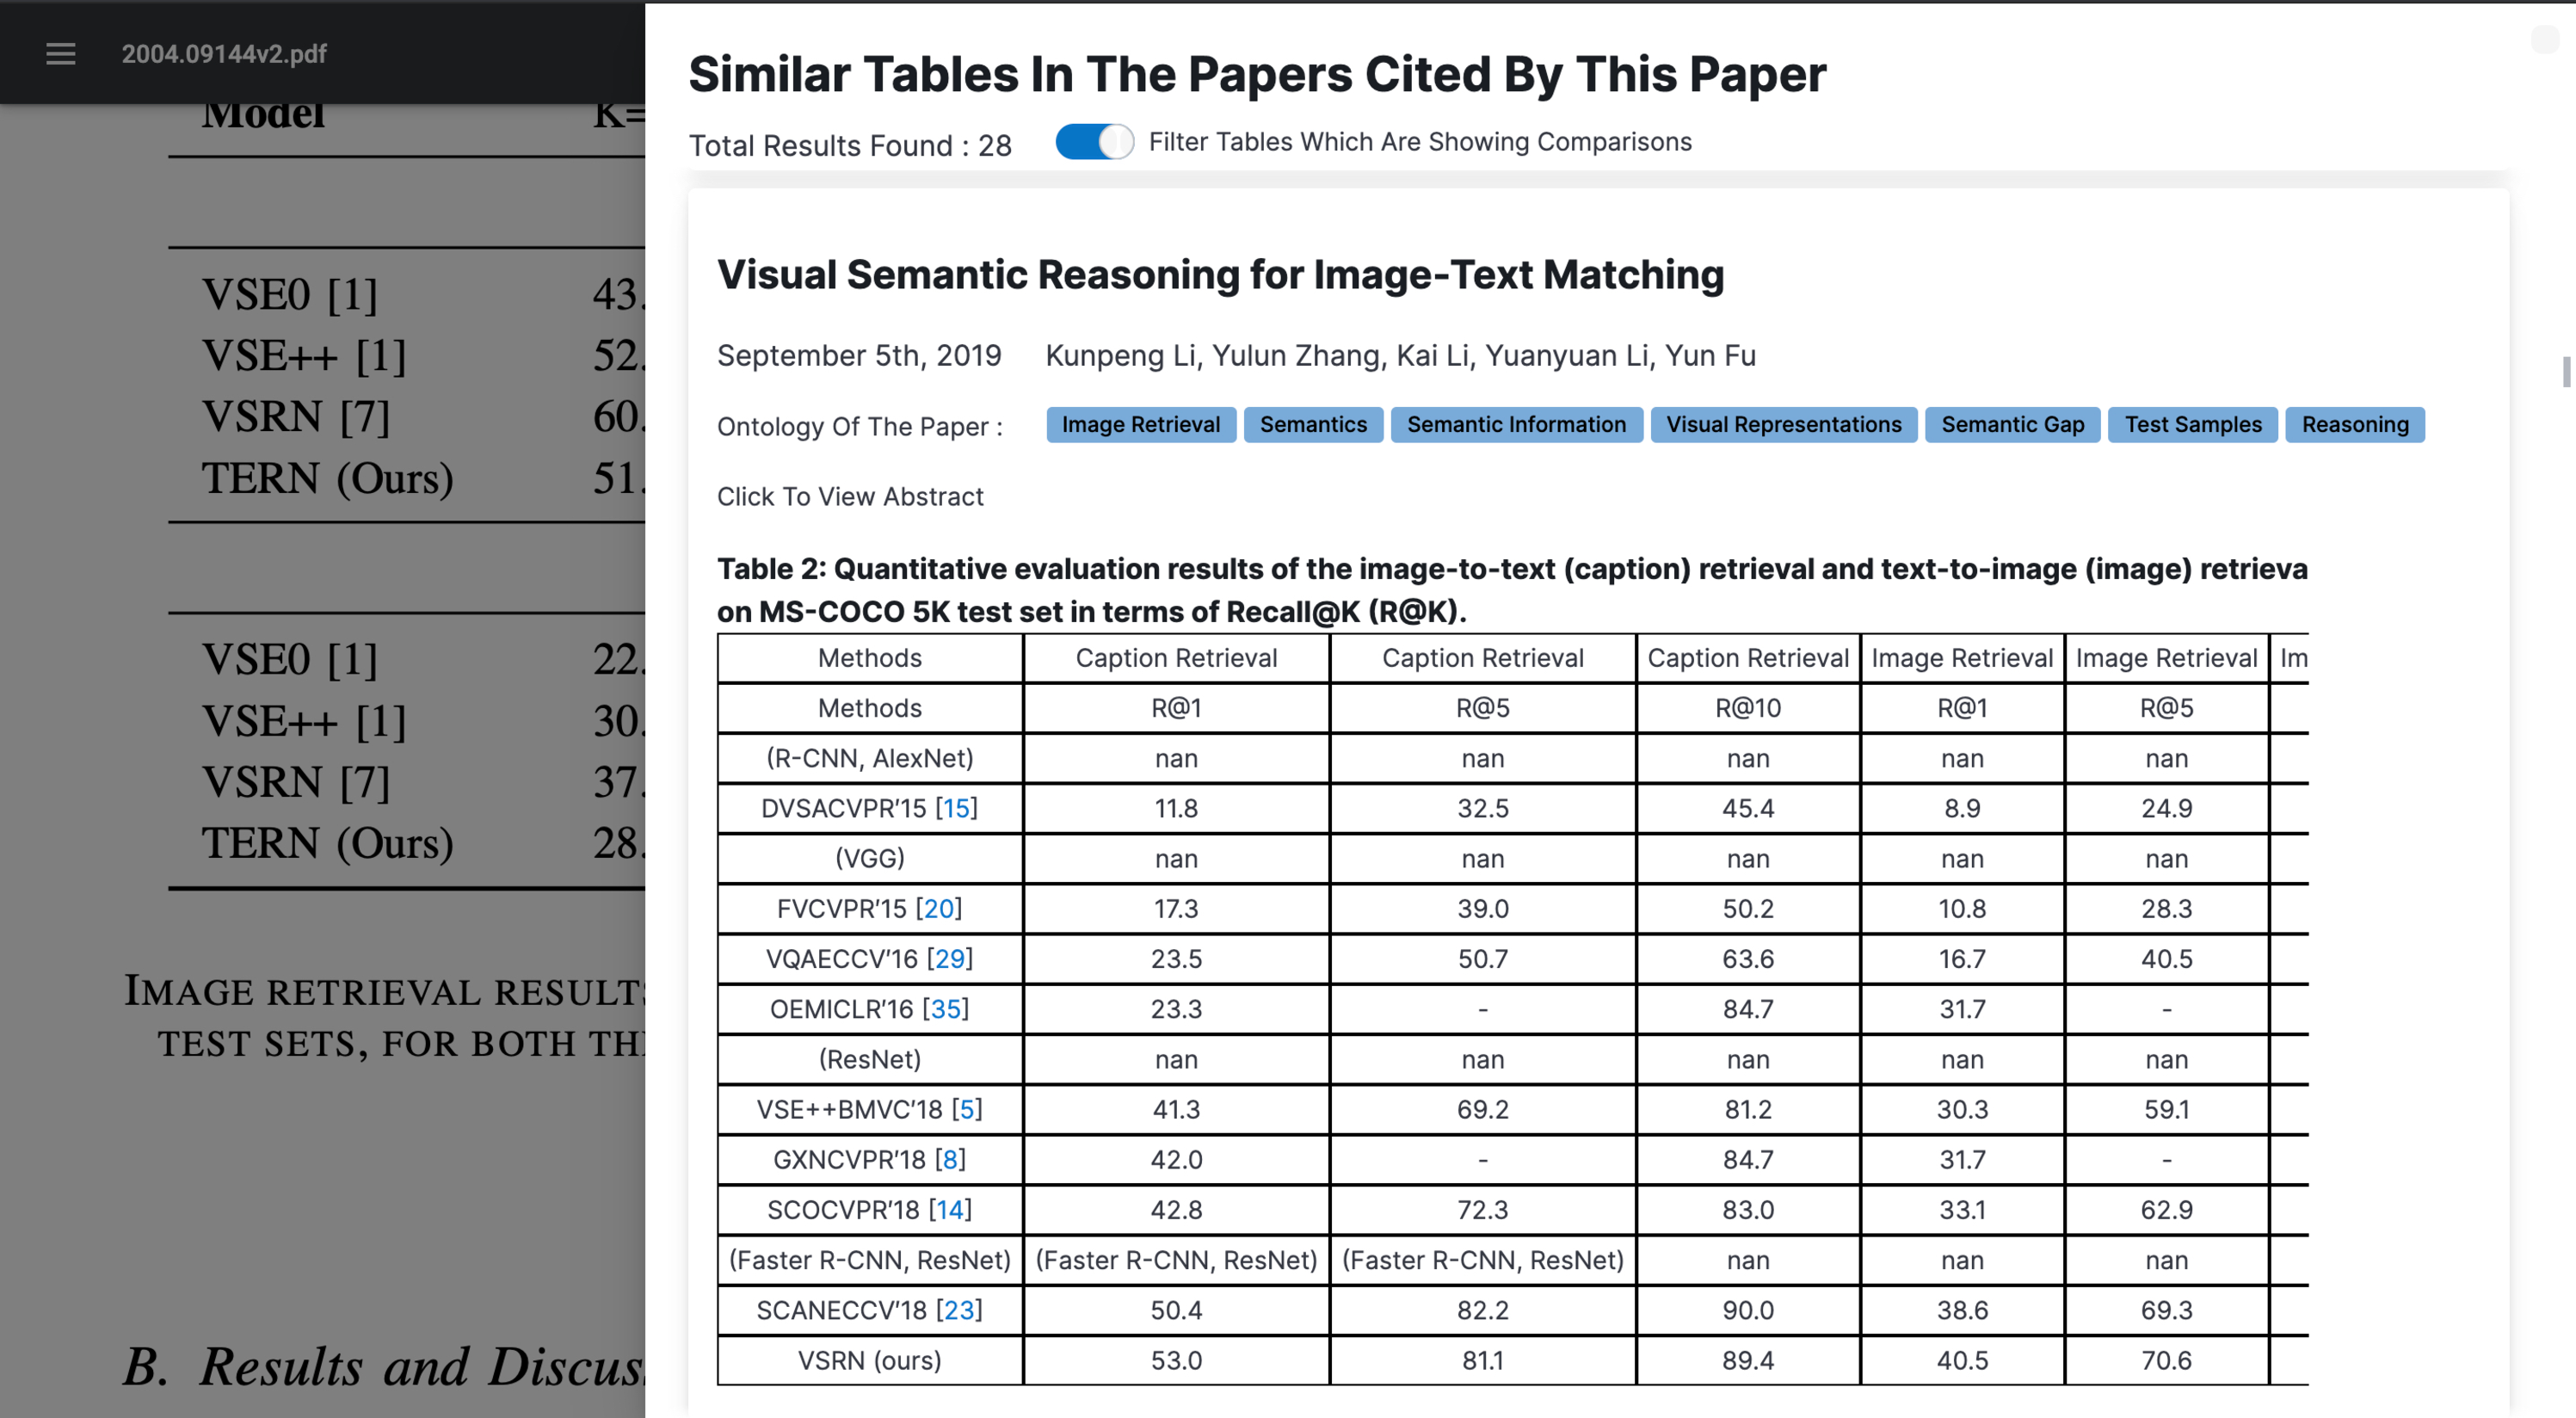
\includegraphics[width=\maxwidth{\textwidth}]{src/images/sci-genie-ext-table-comp-exp.pdf}
    \caption{Sci-Genie Browser Plugin surfacing information about tables comparing entities from cited papers.}
    \label{figure\arabic{figurecounter}}
\end{figure}
\refstepcounter{figurecounter}


\begin{figure}[h]
    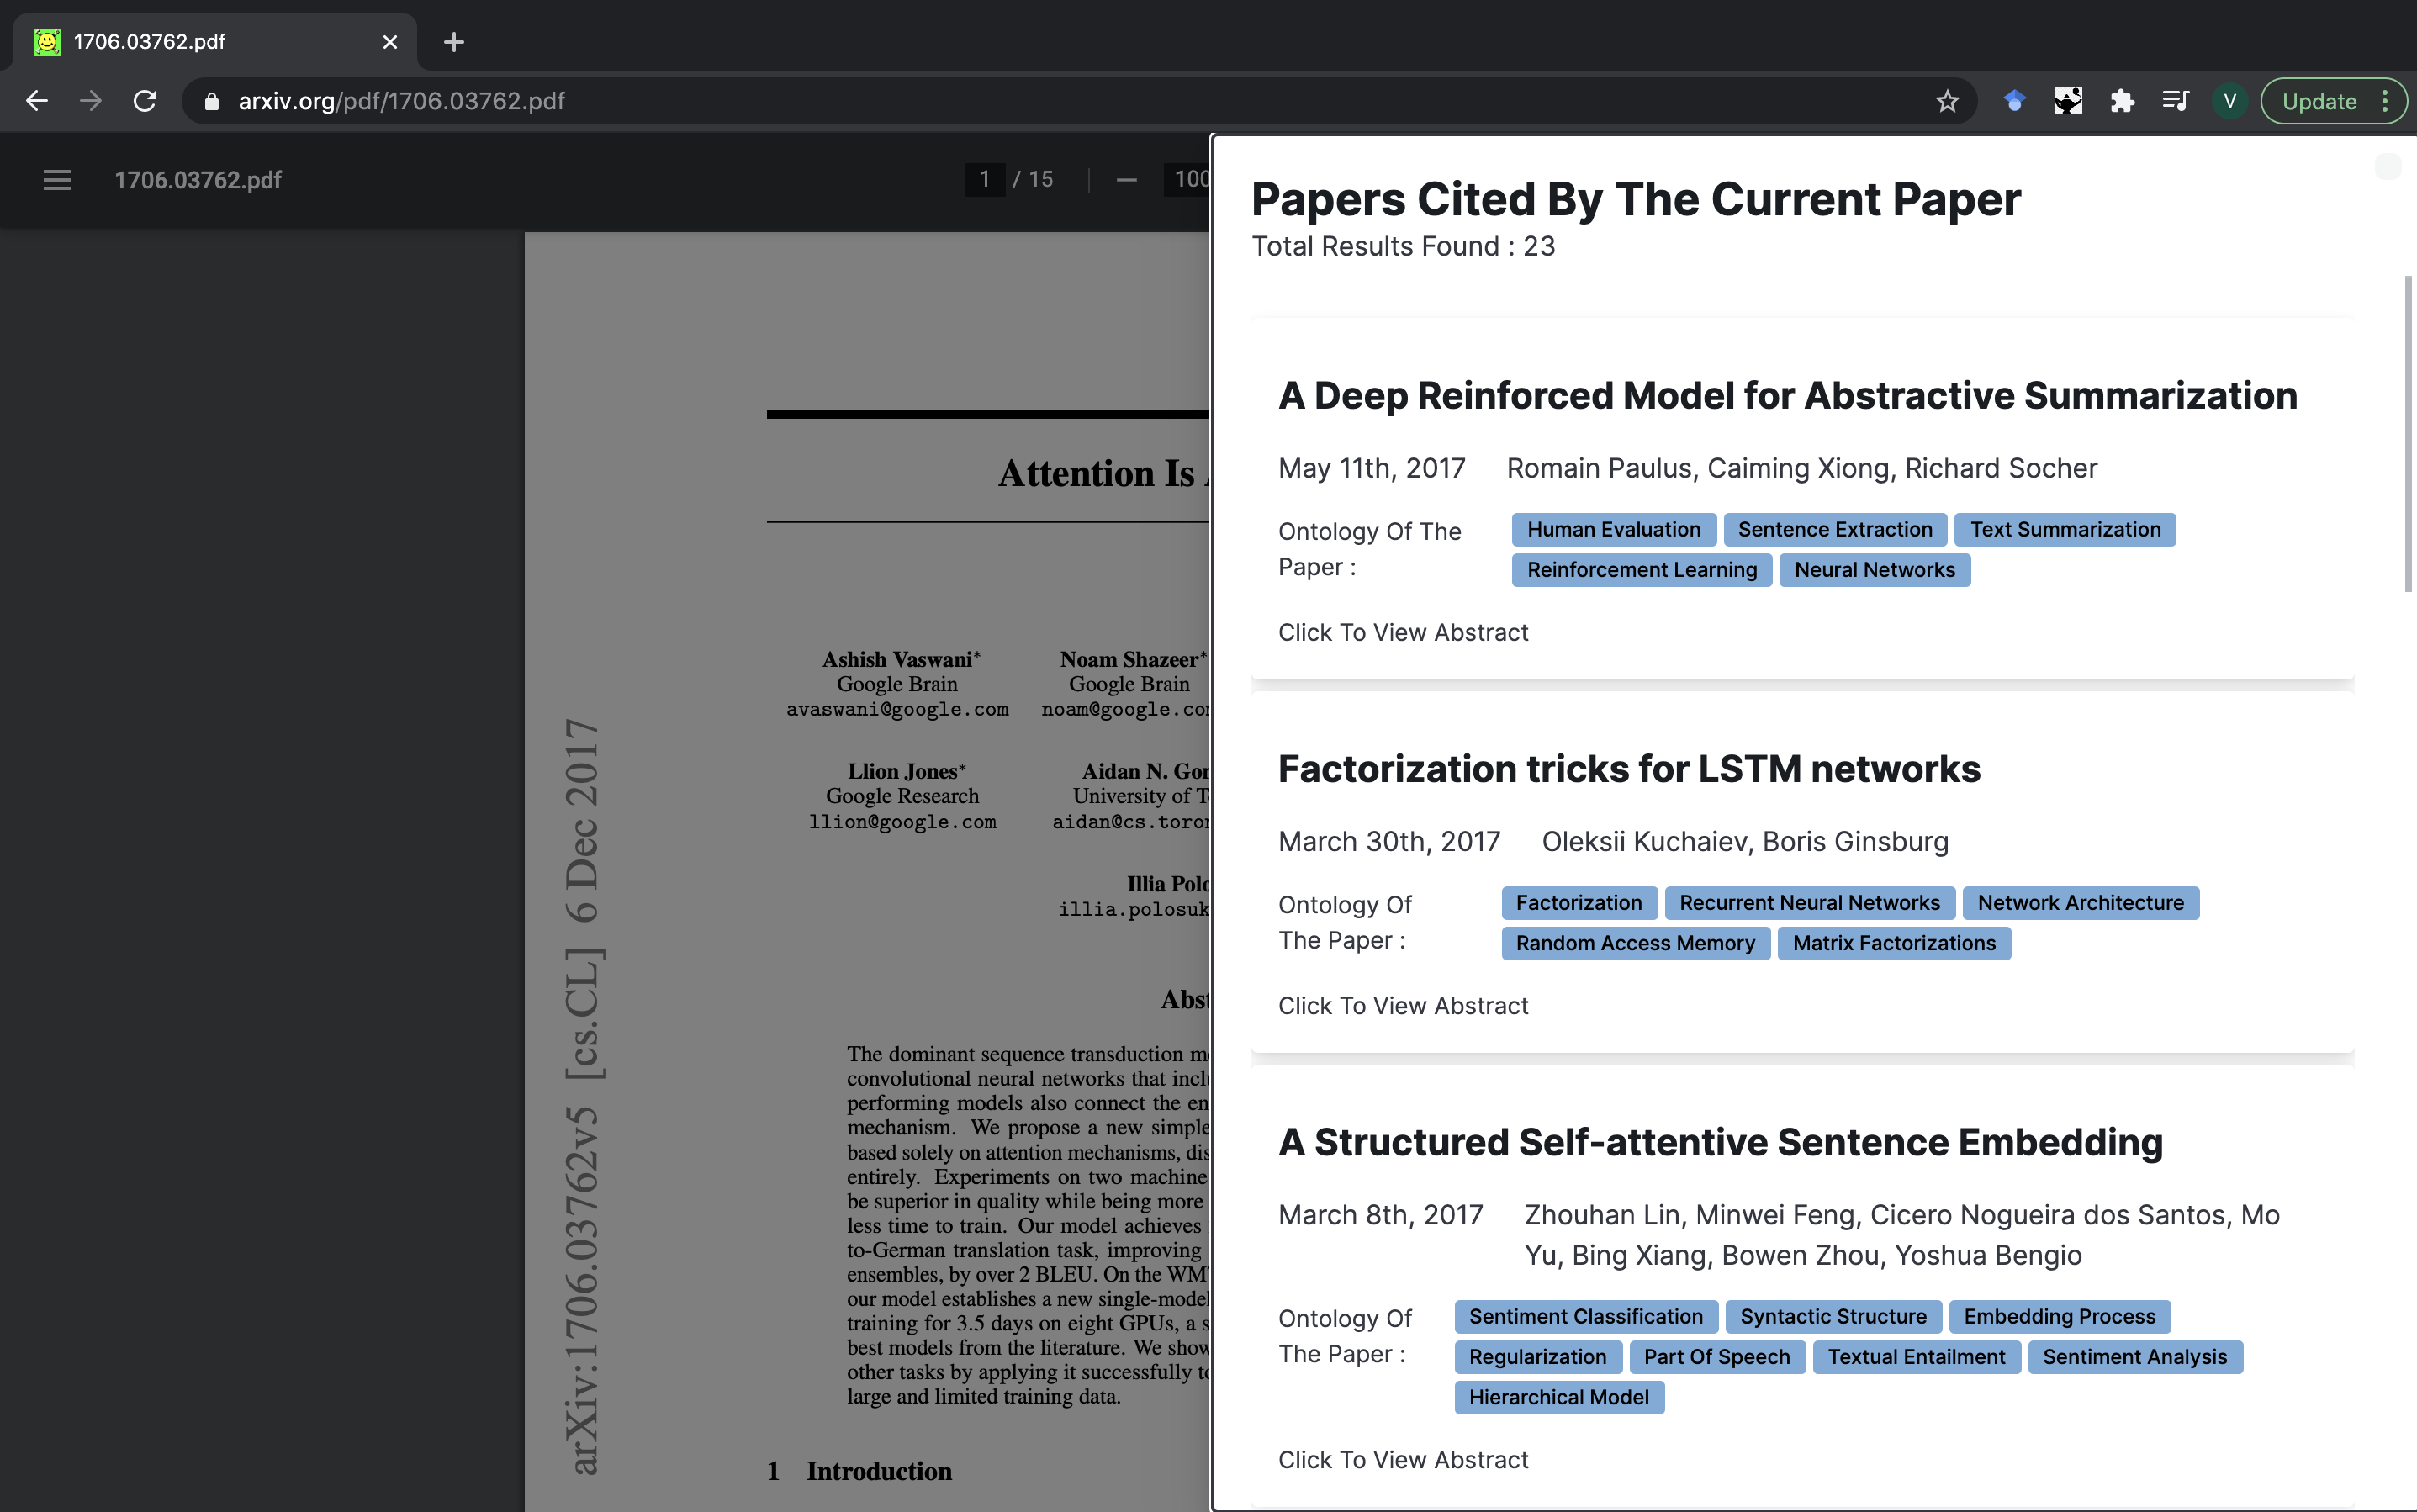
\includegraphics[width=0.475\textwidth]{src/images/sci-genie-ext-cite-out-exp.png}
    \hfill
    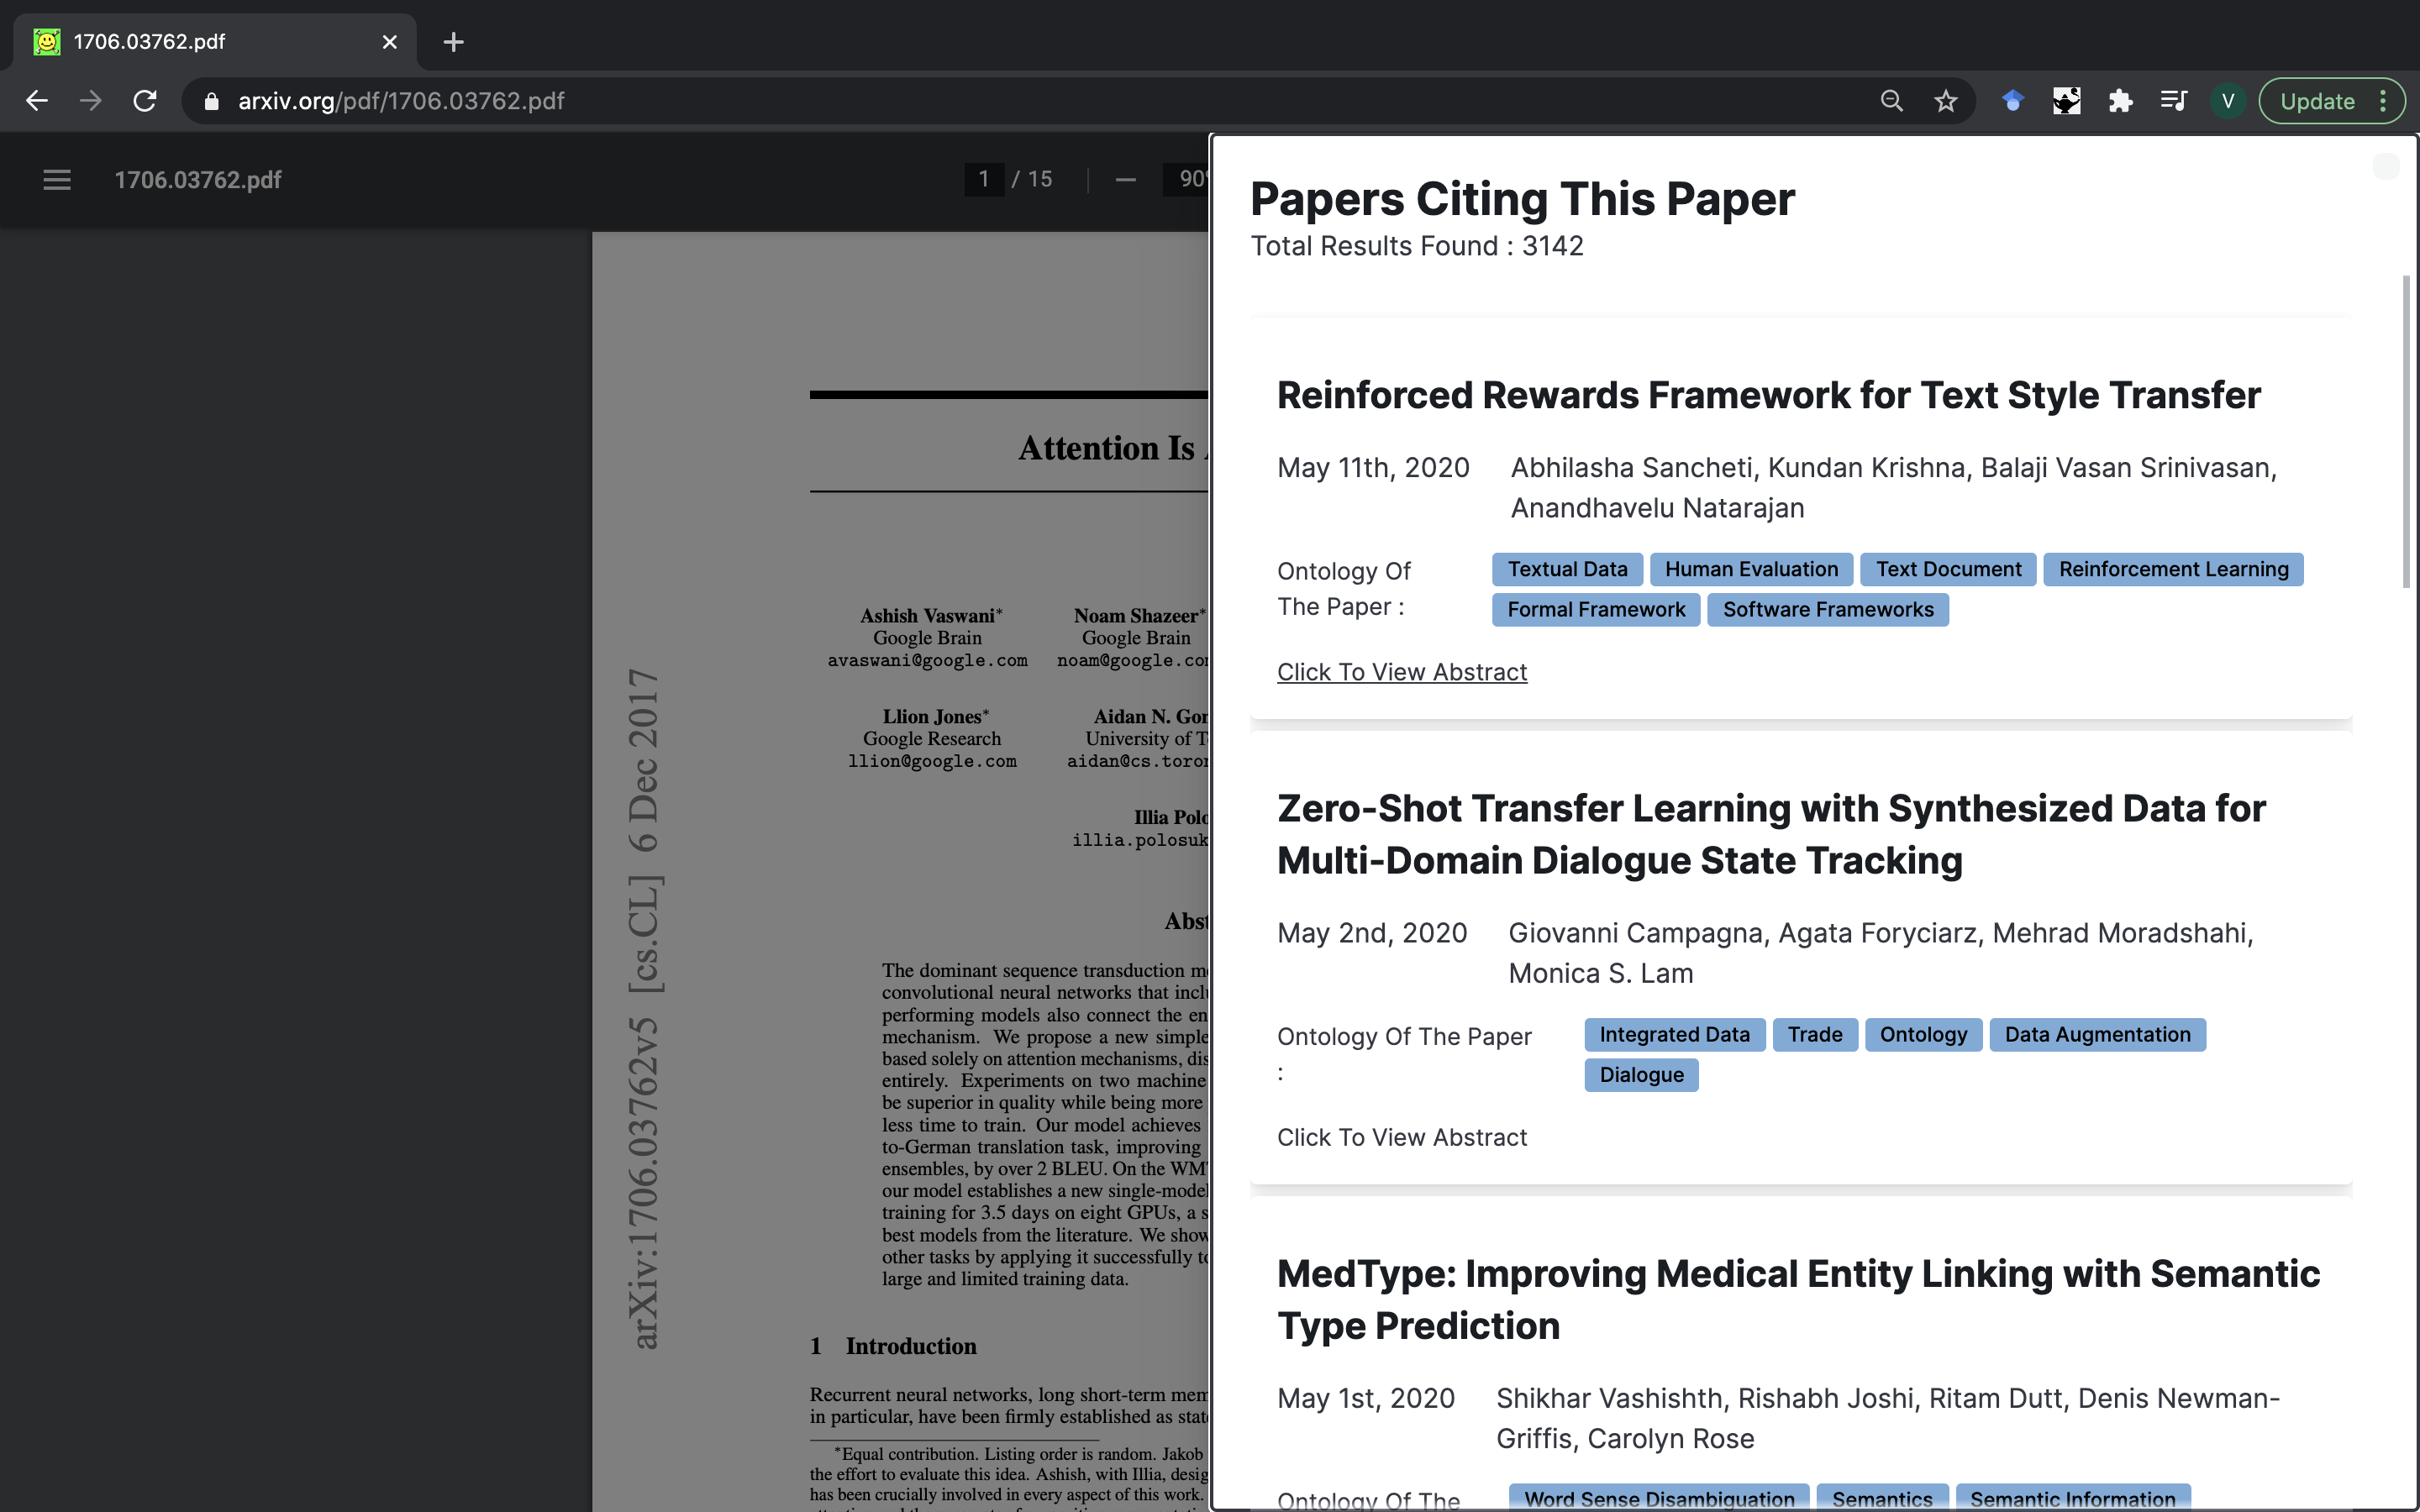
\includegraphics[width=0.475\textwidth]{src/images/sci-genie-ext-cite-exp.png}
    \caption{ Sci-Genie Browser Plugin surfacing context information about papers citing/cited-by the current paper }
    \label{figure\arabic{figurecounter}}
\end{figure}
\refstepcounter{figurecounter}

The citation graph helps surface context-relevant tables from papers cited by the paper the user is reading.  The search engine and the citation graph help extract other papers by the same authors and papers citing/cited by the paper the user reads. Figure \ref{figure10}, \ref{figure11},\ref{figure12}, shows an example of Sci-Genie extension in action. The browser extension also contains filters for filtering tables comparing entities using a machine learning model. All information provided by the browser extension helps enhance the researcher’s understanding without the researcher having to dig up the information independently. 

\begin{figure}[h]
    \centering
    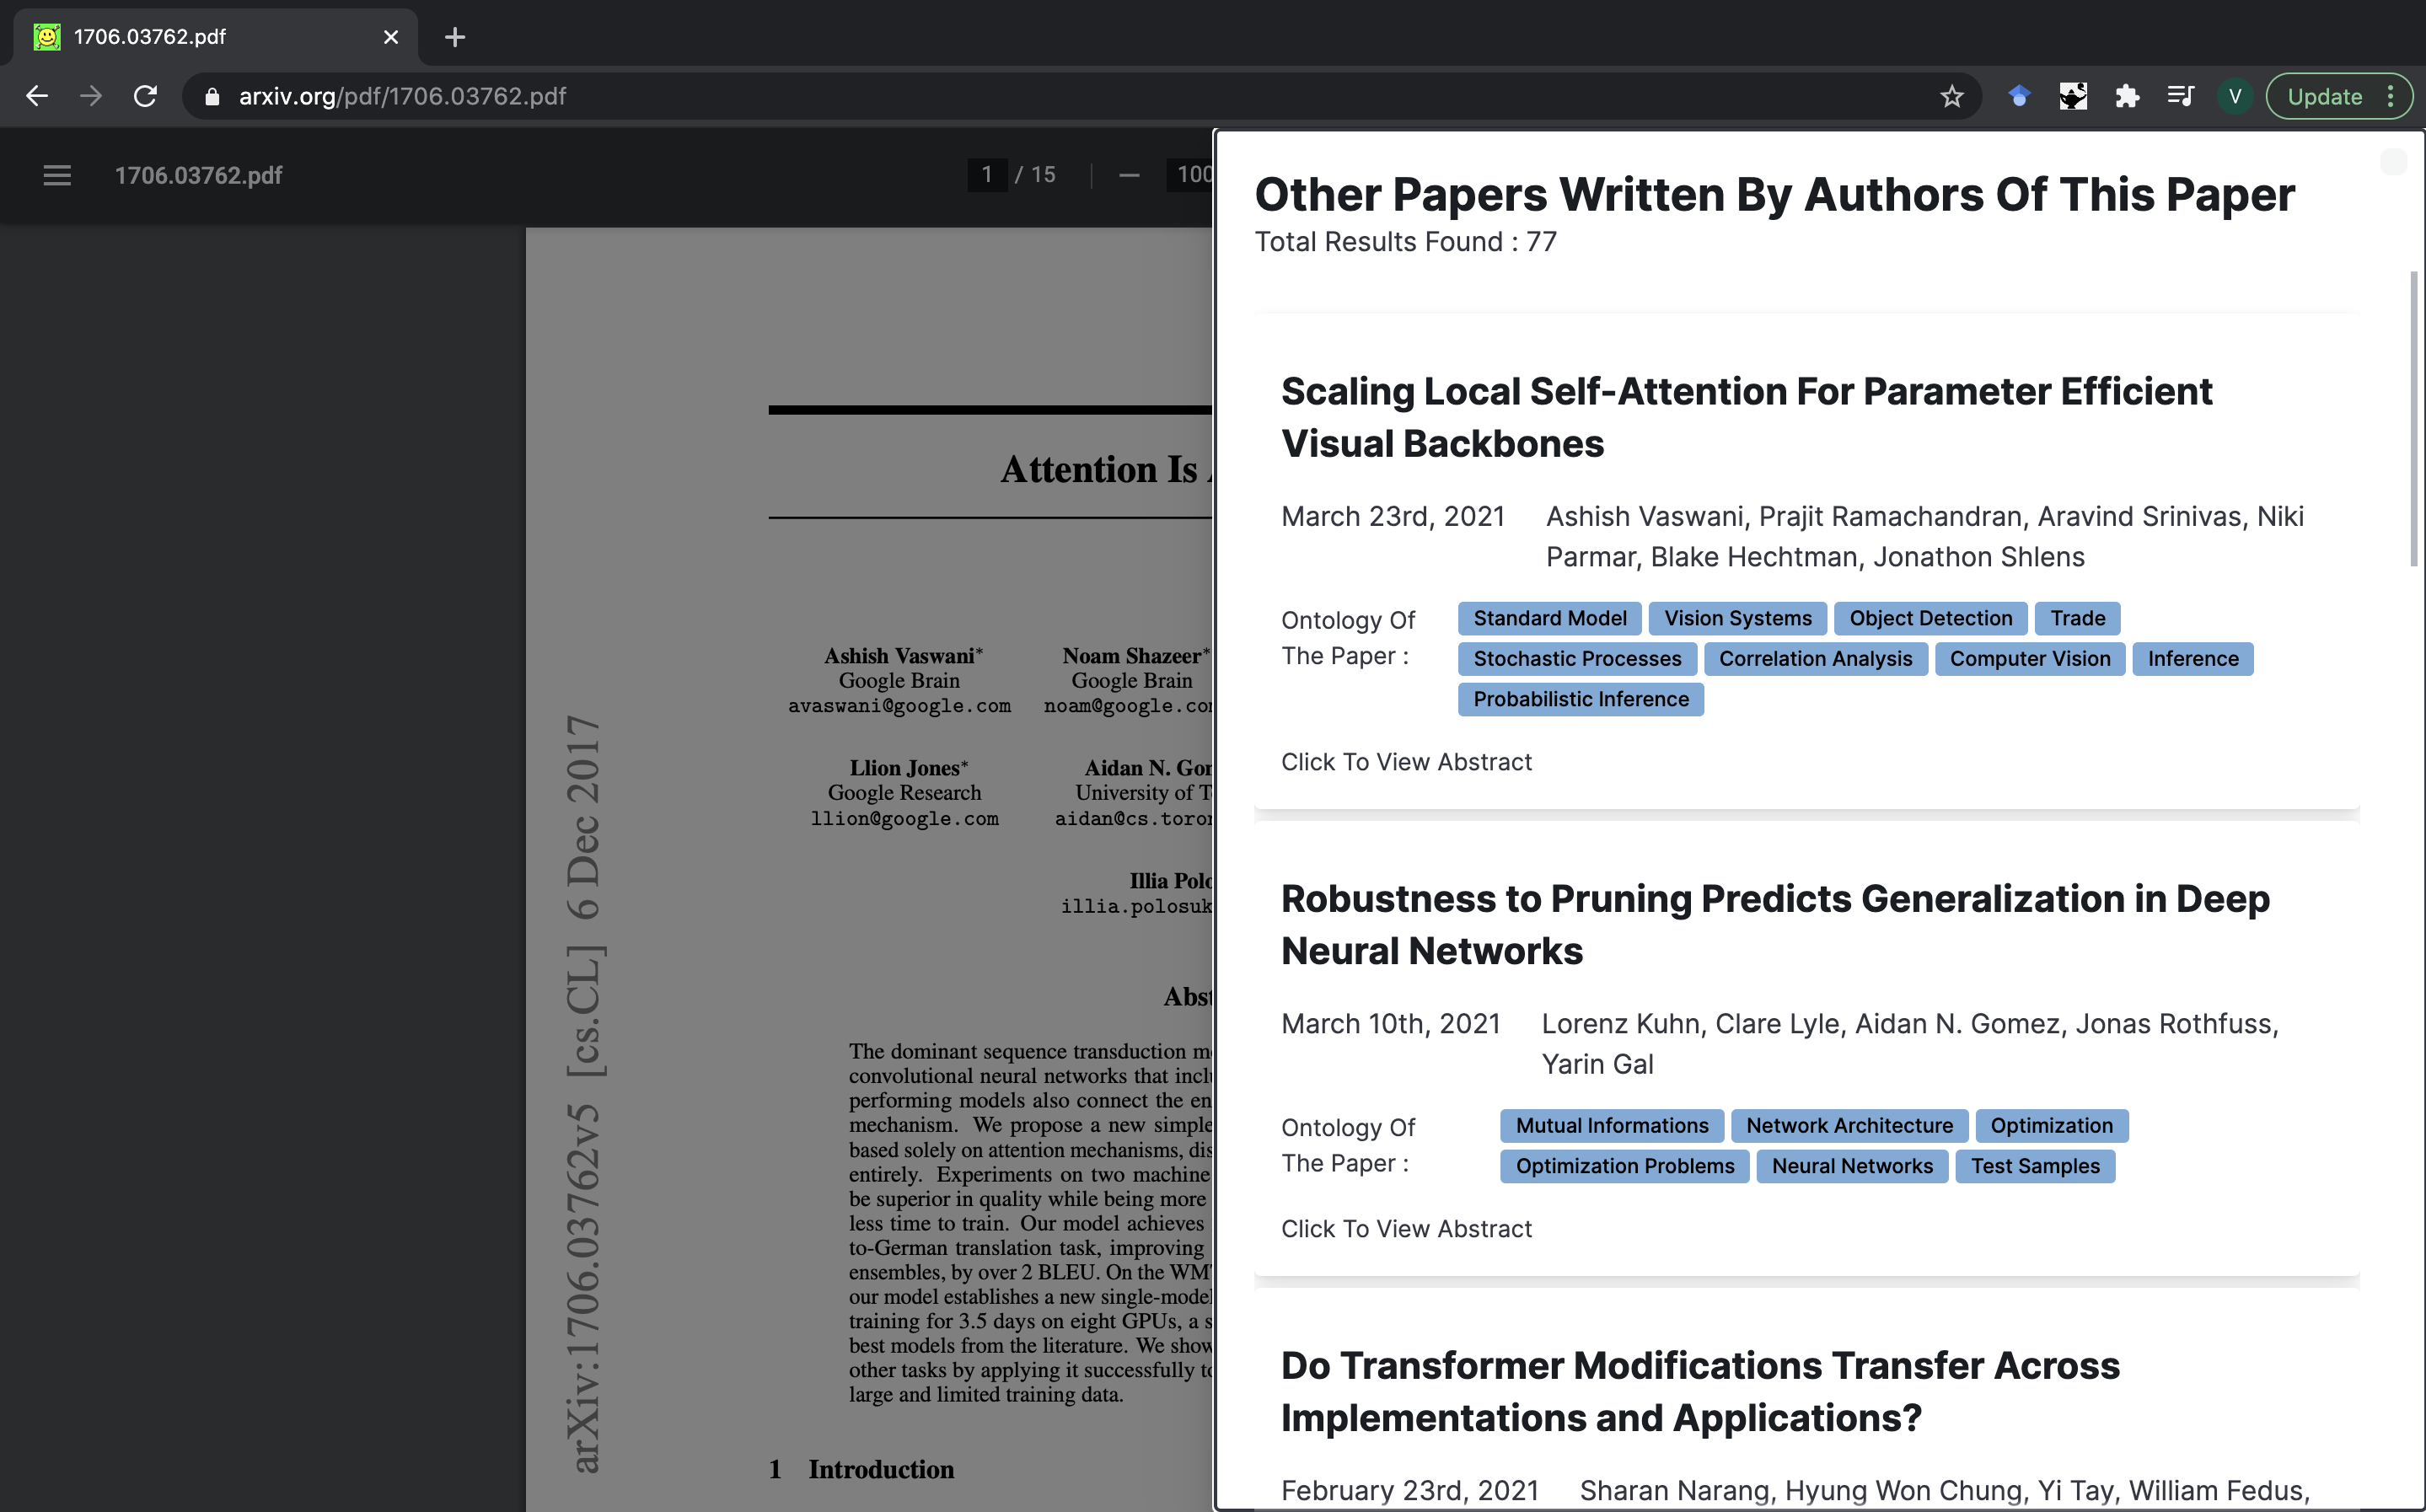
\includegraphics[width=\maxwidth{\textwidth}]{src/images/sci-genie-ext-authors-exp.png}
    \caption{ Sci-Genie Browser Plugin surfacing information about other papers from the authors of the paper the user is reading}
    \label{figure\arabic{figurecounter}}
\end{figure}
\refstepcounter{figurecounter}

\subsection{Design Choices}
Sci-Genie uses ArXiv as a source for papers because ArXiv provides the availability of LaTeX sources. LaTeX based sources are easier to parse compared to PDF documents because of LaTeX's compilability. As LaTeX is Turing complete, the compiled content’s parse tree is easily accessible compared to PDFs. Parsing PDFs is beyond the scope of this dissertation. 